% =====================================================================
% STEPS 3-4 - CROSS-FRAMEWORK DEMAND MAPPING: WHERE TO BUILD FIRST
% Self-contained modular chapter, drafted from the authoritative main.tex
% methodology (§4.5 Phase 3, §4.6 Phase 4, §4.7 Phase 5, §4.8 validation)
% and the Results section (composition + first action points).
% Numbers reconciled to the current dataset (v8 Excel / tool):
%   rows = 33 topics; cols = 31 (30 scored instruments, VSME split);
%   1023 cells, 188 filled (18%);
%   source 12/11/3/5; tiers 12/7/8/4 (VSME=Customer).
% Figures: fig:cell-coding (TikZ, needs tikz+libs in preamble - already in main),
%   topic_distribution.pdf, r_actor_tier.pdf, r_stage_system.pdf.
% =====================================================================

\section{6. Cross-framework demand mapping: where to build
first}\label{angle3-crossmapping}

This chapter covers two steps rather than one. Step~1 (Chapter~4) fixed the
\emph{columns}: the instruments that make up the disclosure ecosystem and how
binding each is. Step~2 (Chapter~5) fixed the \emph{rows}: the disclosure topics
the sector's leading firms actually report, narrowed to a cohort-evidenced
universe.

Step~3, the \emph{overlap}, crosses the two. It scores \emph{who demands what},
topic by topic and instrument by instrument, then reads the resulting matrix for
the thesis's central question: given a fragmented wall of overlapping demands,
which topics satisfy the most of them if built first. Step~4, \emph{building the
tool}, turns that finding into a decision a firm can act on - a short ranked list
of topics to build first, and a diagnostic that tailors the list to its own
situation. Together the two steps answer the third research question and produce
the thesis's central practical contribution.

Figure~\ref{fig:coverage-matrix-screenshot} shows a representative excerpt of the
underlying coverage matrix, so the scale and shape of the raw scoring are visible
before the chapter turns to how it is built.

\begin{figure}[htbp]
\centering
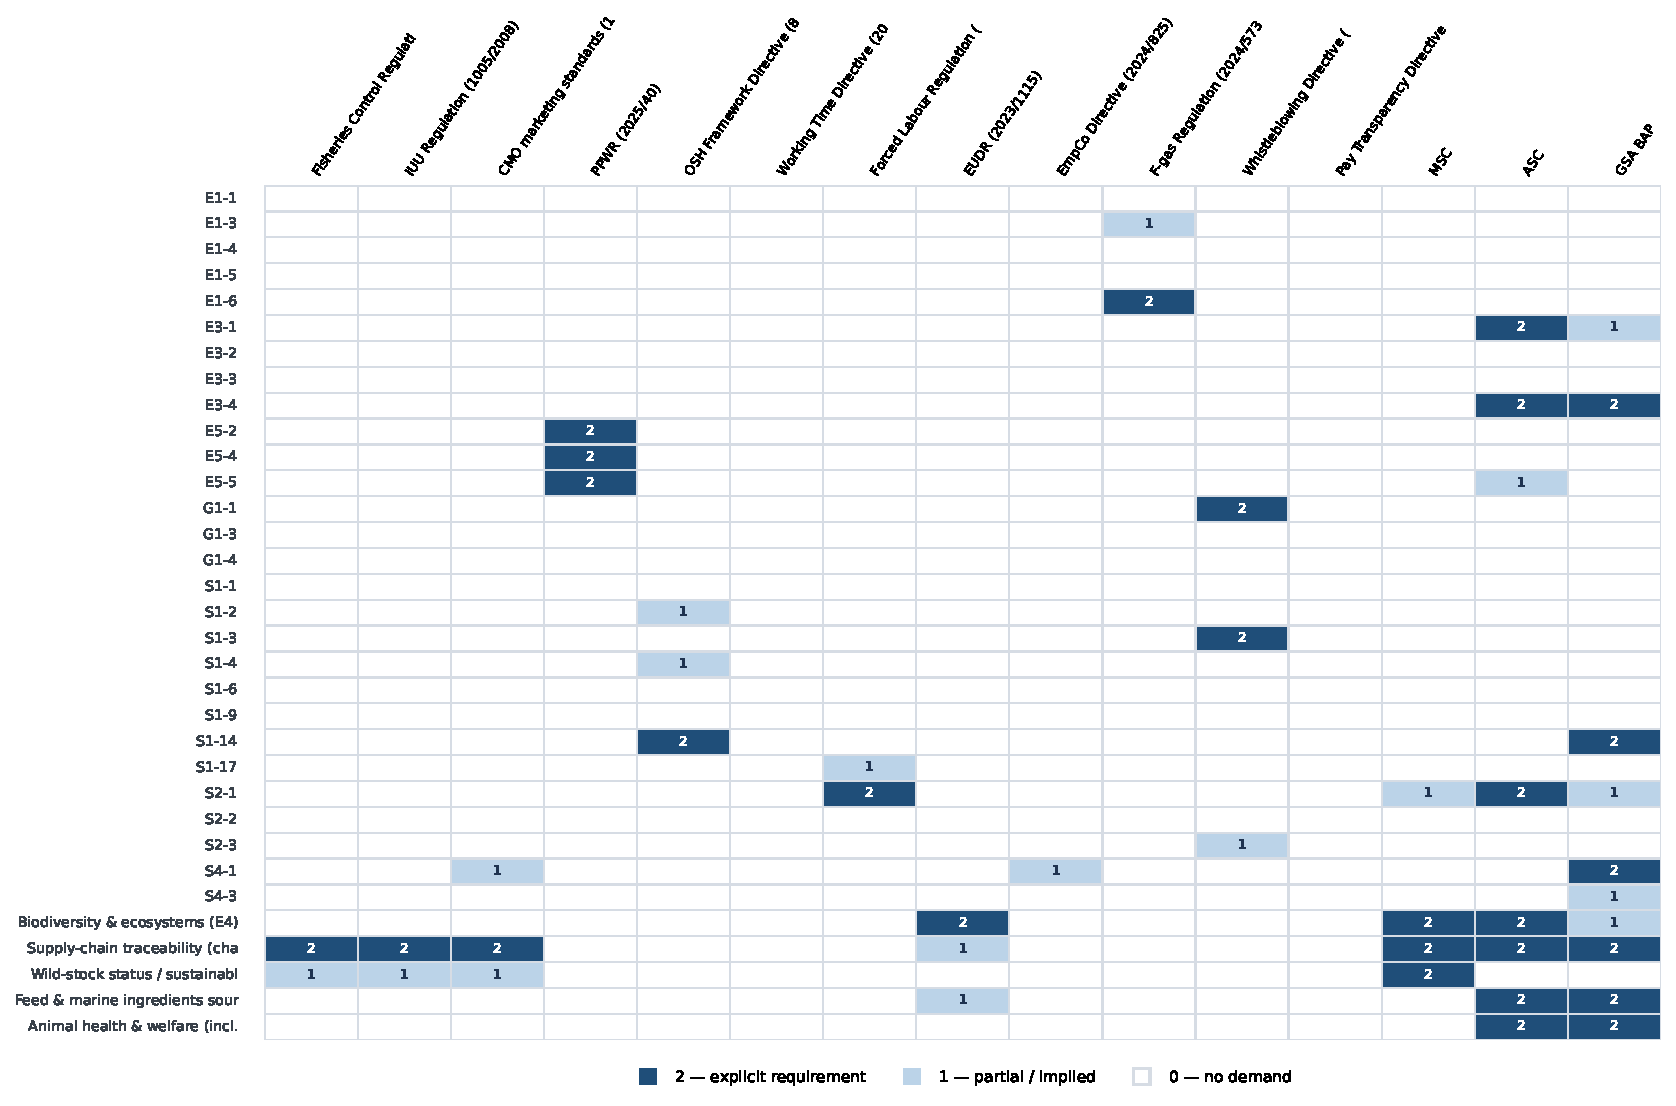
\includegraphics[width=\linewidth]{phase3/appendix_figures/coverage_matrix_screenshot.pdf}
\caption[Representative excerpt of the coverage matrix]{Representative excerpt
of the coverage matrix (\emph{Phase3\_\allowbreak Coverage\_\allowbreak
Matrix\_\allowbreak v18.xlsx}, sheet ``Coverage matrix''): topic rows
against scored-instrument columns, coloured by score (0/1/2). Shows all 33 topic
rows and the first 15 of the 31 scored instrument columns (Tier~1--2); the full
matrix is in the source workbook.}
\label{fig:coverage-matrix-screenshot}
\end{figure}

\FloatBarrier
\subsection{6.1 The convergence logic}\label{cm-theory}

The move from a wall of demands to a short build-first list rests on one idea:
that the demands, though issued by different actors in different vocabularies,
draw on a much smaller set of underlying capabilities, so that a single
capability can answer many demands at once. Two established literatures make this
precise. The first is the \emph{resource-based view} of the firm and the
dynamic-capabilities tradition (Barney, 1991; Teece, 2007), which treat the
ability to produce and reuse structured data as an organisational capability that,
once built, is redeployable across uses at low marginal cost. The second is
\emph{stakeholder-salience} theory (Mitchell, Agle \& Wood, 1997): a firm facing
many legitimate claimants cannot serve each separately and must triage, and the
rational triage is toward the topics on which the most salient claimants converge.
Salience in that account is the combination of three attributes - the
\emph{power} to impose consequences, the \emph{legitimacy} of the claim, and its
\emph{urgency} - and the tiering of Chapter~4 is essentially an empirical reading
of the first two: a Tier~1 legal obligation carries power and legitimacy
together, a Tier~4 voluntary commitment neither. To these three the SME case adds
a fourth constraint that Mitchell's framework treats as given, namely the
\emph{resources} available to answer any claim at all. Triage for a
resource-constrained firm is therefore not only a question of which claimants
matter most, but of how few distinct capabilities the answer can be built from -
which is what the convergence measure below is designed to capture.

Convergence is therefore the organising construct. Where a topic is demanded by a
regulator, an investor framework and an industry standard alike, capability built for that topic is not spent once but several
times over - the compound return that distinguishes a proactive posture from a
reactive one (Chapter~2). A topic demanded through only one channel yields a
narrower return. The analytical task of this chapter is thus to \emph{measure}
convergence across the fragmented landscape and to identify the topics where it is
highest - the hotspots at which building once satisfies many.

\FloatBarrier
\subsection{6.2 Assembling the matrix: rows and
columns}\label{cm-matrix-build}

The matrix has rows and columns, and neither comes straight from the previous
chapters. The rows start from the topics the cohort actually reports
(Chapter~5), which are then trimmed to those the sector agrees on and extended
with four topics the ESRS has no row for. The columns start from the instruments
catalogued in Chapter~4, which are then cut back to those that genuinely ask the
processor for something. Both changes are set out here, before any cell is
scored, because what goes into the matrix decides what it can show: a row for a
topic nobody is asked about, or a column for an instrument that demands nothing,
would distort every count taken from it.

\textbf{Rows: from the cohort frontier to the topic universe.} The rows begin from
the cohort frontier (Chapter~5) and are built up in three steps:

\begin{enumerate}
\item \textbf{The requirements the cohort converges on enter directly} - those
reported by at least five of the six firms. These are the topics the sector's own
practice has revealed to be expected (28 requirement-level rows). The set includes
the climate transition plan (E1-1), which reaches the cut only after the direct
screening of report bodies described in Section~\ref{cohort-method}, because no
GRI disclosure maps to it.

\item \textbf{One topic clears the same bar one level up.} Biodiversity (E4) is
reported by at least five firms when a firm counts as covering the topic if it
reports \emph{any} of the topic's requirements, but no individual E4 requirement
reaches the five-of-six cut on its own - the best-reported reach four. E4
therefore enters as a topic-level row: the same consensus rule at coarser
granularity, not an expert-judgement exception. Consumers and end-users (S4) was
admitted the same way in an earlier version of this analysis; after the bridge
rebuild two of its requirements, S4-1 and S4-3, clear the cut individually, so S4
is now represented at requirement level and needs no topic-level rescue. With the
requirement-level set it forms the cohort-evidenced core (29 rows).

\item \textbf{Four seafood-defining topics have no ESRS home at all} and are
carried in against the GRI~13 sector standard and EU sector legislation:
supply-chain traceability, wild-stock status, feed and marine ingredients, and
animal health and welfare (antimicrobial use folded into the last). These are
flagged as sector-material rather than cohort-evidenced. Each carries a
production-system tag - wild, aqua or both - so a firm drops the rows that do not
concern it.
\end{enumerate}

The funnel therefore runs from the 70 topical ESRS disclosure requirements, narrows
to the cohort-evidenced core, then \emph{extends} by four. Those four are the one
place where the ESRS blueprint is insufficient and the sector standard supplies the
rows instead. Stated as a sequence, with each figure used once:

\begin{enumerate}\itemsep2pt
\item \textbf{70} topical ESRS disclosure requirements form the starting universe
(Chapter~5).
\item \textbf{28} of those are reported by at least five of the six firms at
requirement level, and enter directly. E1-1 is among them, reached through the
body screening of Section~\ref{cohort-method} rather than through the bridge.
\item \textbf{+1} topic-level row, biodiversity (E4), where the topic clears the
consensus cut but no single requirement within it does - giving \textbf{29}
cohort-evidenced rows.
\item \textbf{+4} sector-material rows carried in from GRI~13 and EU sector law,
for which no ESRS requirement exists: supply-chain traceability, wild-stock
status, feed and marine ingredients, and animal health and welfare.
\item \textbf{33} rows in total, scored against \textbf{31} instrument columns -
30 instruments, with the VSME split into its Basic and Comprehensive modules -
giving the \textbf{1{,}023} cells of the matrix.
\end{enumerate}

They are not chosen ad hoc. Each of GRI~13's 26 material topics
(Agriculture, Aquaculture and Fishing) was classified against the ESRS as
\emph{covered}, a \emph{reporting gap} (an ESRS mapping exists, but cohort
reporting on it falls below the $\geq$5/6 consensus threshold), or a
\emph{structural gap} (no ESRS disclosure requirement exists at all).

The four divide evenly between two of those categories. Animal health and welfare
and supply-chain traceability are structural gaps: the ESRS has no requirement
covering either, so nothing in the standard asks for them at all. Wild-stock
status and feed and marine-ingredient sourcing are different. Both are
production-specific disclosures nested inside biodiversity (GRI~13.3), which is
itself covered and already in the universe. The broad subject is therefore
present, but these two specific disclosures within it are not. The full
classification is given in \nameref{app:gri13}.

\textbf{Columns: from the full ecosystem to the scored instruments.} The columns
begin from the instruments catalogued in the ecosystem (Chapter~4). That
catalogue is deliberately the whole field, so it includes instruments that place
no scorable demand on the processor in the end. The scored set is the subset that
does.

Three groups are set aside. The \emph{context} instruments bind Member States
rather than the firm. The \emph{excluded} instruments fail the second of the two
admission gates screened at catalogue stage - ESG relevance first, then
organisation-level obligation - which are defined and applied instrument by
instrument in \nameref{app:scope}. The CSRD/ESRS standard is held out separately
as the \emph{baseline} reference against which the rows are defined, rather than
scored as one more demand.

That leaves \textbf{30} scored instruments. Only one of them, the VSME, is split
into two columns, for its Basic and Comprehensive modules, because it is the only
instrument with two officially defined and nested reporting tiers - which is why
30 instruments occupy 31 columns. Each scored column inherits its stakeholder
source and its obligation locus (direct, indirect or context) from Step~1. Some columns are switched off for a given firm because its profile puts
the instrument out of scope, and two kinds of switch apply. The first is the
production system: a wild-only firm switches off the aquaculture certifications
(ASC, BAP). The F-gas switch is separate from production system and turns on
equipment rather than sourcing: it is switched \emph{on} for the modelled firm,
since refrigeration is near-universal in seafood processing, and exists only for
the minority of sites that have already converted entirely to natural
refrigerants such as ammonia or CO\textsubscript{2} and hold no fluorinated gas.
The second switch is size: within the SME band several obligations turn on
headcount - the Pay Transparency Directive's gender pay-gap reporting applies from
150 employees and the whistleblowing obligation from 50 - so a firm below a
threshold switches off the instruments above it. A switched-off instrument is
excluded from that firm's demand sums, though a customer may of course still ask
for the same content contractually, in which case the demand reaches the firm
through the customer channel rather than the legal one. The full
instrument-by-instrument classification - scored, baseline, context or excluded,
with the reason for each - is provided in \nameref{app:scope}.

The demand matrix is therefore a grid of topic rows against instrument columns,
every cell recording how strongly a given instrument demands a given topic, on the
scale set out next.

\FloatBarrier
\subsection{6.3 Scoring the matrix}\label{cm-matrix}

\textbf{The coverage scale.} Each cell is coded on a three-level scale defined ex
ante:
\begin{itemize}
\item \textbf{0 - not covered:} the instrument does not address the topic, or its
demand maps only to datapoints outside the row universe (the out-of-frame rule
below).
\item \textbf{1 - touched:} the instrument references the topic but imposes no
binding requirement on any of its datapoints.
\item \textbf{2 - required:} the instrument explicitly and bindingly requires
the entity to achieve, address, comply with, certify, report on or disclose at
least one datapoint belonging to the topic.
\end{itemize}
Binding \emph{conformity} counts equally with binding \emph{disclosure}: a
mandatory recycled-content target (e.g.\ the PPWR), an accident-prevention duty
(e.g.\ the OSH Framework Directive) or a market-access prohibition on
forced-labour products (e.g.\ the Forced Labour Regulation) scores~2 even where
no report is filed, because it bindingly addresses the datapoint substance. The score
measures \emph{how strongly} an instrument demands a topic; it says nothing about
\emph{how} that demand reaches the firm, which is a different question. A demand that
arrives indirectly - CSDDD, which for the sub-threshold processor modelled here
binds its large customers and reaches it as a cascaded supplier requirement,
though it would bind a larger processor directly - is still scored on its
strength: if
it bindingly imposes a topic's datapoints it scores~2, exactly as a directly binding
rule would. Whether the route is direct or indirect is recorded separately, as the
obligation locus, and never raises or lowers the score. Keeping the two apart stops
an indirect-but-binding demand from being under-counted merely because it is
transmitted rather than imposed.

\textbf{Datapoint-grounded coding.} A score is assigned against the
\emph{constituent datapoints} of a requirement, not against the title of its
disclosure requirement. Each of the 29 cohort-evidenced rows is decomposed into
its official EFRAG datapoints using the ESRS datapoint master (Commission
Delegated Regulation (EU) 2023/2772): the 26 DR-level rows resolve to 356
datapoints and the two topic-level rows (E4, S4) to a further 152. An instrument
scores~2 where its indicators demand at least one of a requirement's datapoints,
1 where it references the topic but demands none of them, and~0 where it is
silent. This replaces the broad question of whether instrument~$f$ addresses
topic~$r$ with the concrete and reproducible one of whether~$f$ demands at least
one datapoint of~$r$. It also surfaces corrections. Whistleblowing demand, for
instance, resolves to the governance row that actually carries the whistleblowing
datapoints rather than to an adjacent anti-corruption row. Once such corrections
are logged they are findings about the coding process rather than matters of
method.

\textbf{When self-reporting counts as a binding demand.} Many instruments are
self-reported, which raises a scoring question with real consequences: whether
completing a supplier questionnaire places the same demand on a topic as reporting
against a defined standard. Treating the two alike would inflate the matrix, so a
single rule separates them - and what matters is not \emph{who} reports but whether
the \emph{datapoints are fixed in advance}:
\begin{itemize}
\item An \emph{open-question self-assessment}, where the firm describes itself
against broad prompts with no defined datapoints and no external threshold
(e.g.\ EcoVadis, the Sedex SAQ), shows the topic is relevant to the firm but
pins down no specific data. It scores~\textbf{1}.
\item A \emph{defined-datapoint standard}, where the datapoints to report are fixed
ahead of time - voluntary (GRI, CDP, TNFD) or mandatory (the ESRS) - imposes the
datapoint even though it too is self-reported. It scores~\textbf{2}.
\item An \emph{enforced-conformity} requirement, where the firm must meet a bar and
fix failures (a SMETA audit it must pass to keep the buyer, or a binding legal duty),
likewise scores~\textbf{2}.
\end{itemize}
A last line separates a rating the firm \emph{feeds} from one built \emph{about} it:
a rating is scored only where the firm must supply the data itself (EcoVadis,
scored~1); purely external ratings assembled from public data (MSCI, Sustainalytics,
the Dow~Jones Best-in-Class Indices) place no demand on the firm and are not scored
at all, since such a rating consumes disclosures rather than asking for them.

\textbf{Sector-material rows.} For the four seafood-specific gap rows
(traceability, wild-stock status, feed and marine ingredients, animal health and
welfare) no ESRS datapoint exists by construction; these are scored against the
criteria of the demanding instruments themselves - MSC Principle~1 stock-status
reference points for wild-stock, the GDST key data elements for traceability, and
ASC antibiotic and survival criteria for animal health and welfare. A pinned rule
prevents double-counting on the wild-stock/E4 boundary: stock-status and
legal-sourcing demand (MSC Principle~1, the IUU catch-certificate regime) codes
to the wild-stock row, whereas generic biodiversity and
ecosystem-impact demand (ESRS~E4, GRI~101, TNFD, MSC Principle~2 on bycatch and
habitat) codes to E4; a single instrument may legitimately score on both rows
through different provisions.

These four rows are not equivalent kinds of measure, and the distinction matters
for how their scores should be read. Wild-stock status is an \emph{outcome}: it
asks whether the stock a firm buys from is healthy, and answering it requires
stock assessment science and reference points the processor does not generate
itself. Supply-chain traceability is an \emph{assurance mechanism}: it
establishes that a product came from where it is claimed to have come from, and
says nothing on its own about whether that source is sustainable. A firm can
operate complete traceability on a stock that is severely overfished. The high
demand score traceability carries in this matrix therefore records how many
instruments require it, not that meeting it evidences a sustainability outcome.
The two rows are kept separate for exactly this reason, and the build-first
ranking that follows should be read as a map of what the environment
\emph{asks for} rather than of what most improves the state of the resource.

\textbf{Are wild-stock status and traceability actually live practice, not
just a GRI category?} Neither has an ESRS DR, so neither was captured by the
cohort's DR-level coverage coding in Chapter~5 - which raises a fair
question: is including them here just following GRI~13's classification, or
is there evidence the sector's own leading firms actually treat them as
real, active topics? All six cohort firms do, on both counts
(Table~\ref{tab:sector-material-evidence}).

\begin{table}[H]
\centering
\caption{Sector-material topics in the cohort's own reporting. Each firm
discloses both a sustainable wild-sourcing certification level and a
traceability system, though neither topic has an ESRS disclosure requirement.
Figures as published by each firm; wording follows the source report.}
\label{tab:sector-material-evidence}
\footnotesize
\begin{tabularx}{\textwidth}{@{} l X p{4.5cm} @{}}
\toprule
\textbf{Firm} & \textbf{Sustainable sourcing, as reported} & \textbf{Traceability} \\
\midrule
Thai Union (2024) & 98.9\% of tuna MSC-certified, in MSC assessment, or FIP-covered & Working toward GDST compliance \\
Bolton (2024) & 99.7\% of tuna from responsible fishing practices: MSC-certified, in full MSC assessment, or covered by a credible and comprehensive FIP & Working toward GDST compliance \\
Nomad Foods (2025) & 99.9\% of fish and seafood certified sustainable or responsibly sourced & Own digital traceability system \\
Espersen (2025) & 99\% of fish and seafood sourced in accordance with third-party certification & Own electronic traceability system \\
Mowi (2025) & 100\% of harvest volume certified to a GSSI-recognised standard (ASC, BAP or GLOBALG.A.P.) & Own digital traceability system \\
Profand (2025) & MSC- and ASC-certified sourcing & Active GDST participant \\
\bottomrule
\end{tabularx}
\end{table}
The figures in the middle column are not comparable across firms and are not
used comparatively here. Each firm defines its own numerator: some report
certified volume alone, others bundle certified volume with product in
assessment and with fisheries covered by improvement projects, and some state a
figure for one species rather than the whole portfolio. The column records that
each firm makes a sourcing claim and on what basis, not how the firms rank
against one another; no claim in this thesis rests on the difference between
99.9\% and 98.9\%.

The two topics fall outside the ESRS structure this thesis uses as its main
coordinate system, but they are not a marginal or invented addition: every
firm in the cohort reports on both, independently of each other and of GRI~13's
classification. This is stated here as corroboration, not as scored
evidence - these mentions were not coded against a defined datapoint set
the way the 70-DR cohort analysis was, so no coverage percentage is claimed
for them.

\textbf{Does this reach a firm that only processes, not farms or fishes?} A
pure processor buys already-caught or already-farmed product; it does not
manage a stock or run a farm. So how much of the wild-stock, feed and
animal-welfare demand above actually lands on it? All of it, but in two
different ways, and the matrix tags which is which. \emph{Direct}: the
processor itself holds a Chain-of-Custody (CoC) certificate (MSC, ASC,
GLOBALG.A.P., BAP, Friend of the Sea) and keeps its own segregation and lot
records to prove it - this is an obligation on the processor itself.
\emph{Indirect}: to hold that CoC certificate at all, its supply contracts
must specify sourcing from a stock, farm or feed mill that meets the
scheme's upstream standard - for instance MSC Principle~1 on stock health, or
ASC's feed and antibiotic limits. These are illustrative rather than exhaustive:
both schemes are full standards, and a supplier is certified against the whole
of one, not against a single principle. MSC covers stock status, environmental
impact and management system across its three principles, and ASC likewise
extends well beyond feed; no buyer accepts conformity with one principle alone.
The examples are named here only because they are the clauses through which the
upstream demand reaches the \emph{processor}.

This transmission also runs in the other direction, which qualifies the common
assumption that a processor is simply a demand-taker. A purchasing policy that
specifies certified sourcing exerts real pressure upstream, and a large enough
book of such policies can move a fishery: the Argentine hake fishery
(\emph{Merluccius hubbsi}) has moved toward MSC assessment in response to buyers
declining uncertified product (O.~Spring, Group Sustainability Manager, Nomad
Foods, personal communication, August 2026). The effect is weaker for a single sub-threshold SME than for a
large buyer, but it is not absent, and it is one route by which a small
processor's disclosure capability converts into influence rather than only cost.

The processor doesn't manage the upstream operation, but
it cannot keep its certificate without sourcing from one that does - so
the demand is real, just transmitted rather than performed directly. Each
cell is scored on the same 0/1/2 strength scale either way (a core
criterion such as MSC~P1 stock status or ASC feed-conversion limits scores~2,
a lighter good-practice mention~1); direct or indirect only records \emph{how}
the demand reaches the processor, and - as stated above - never changes the score itself.

One locus tag needs qualifying. EUDR's due-diligence duty on feed and
marine-ingredients sourcing binds the feed manufacturer importing raw soy or
palm, not a processor further downstream buying finished feed. For the modelled
sub-threshold processor the demand therefore arrives indirectly, through the feed
supplier's own compliance. The source workbook records obligation locus once per
instrument column rather than per cell, so EUDR carries a single \emph{direct}
tag there; the qualification stated here applies to the feed row specifically.
Because locus is descriptive and never enters the score, no coverage figure in
this chapter is affected.

\textbf{Out-of-frame demand.} Some indicator-level demand maps cleanly onto an
ESRS datapoint that lies \emph{outside} the cohort-defined universe: the Pay
Transparency Directive's gender pay-gap requirement maps to S1-16, the Working
Time Directive to S1-11/S1-15, none of which cleared the $\geq$5/6 consensus and
so have no row. Such demand scores~0 against the in-universe rows and is
\emph{not} reassigned to the nearest available row (which would misattribute and
inflate it); instead it is recorded in a separate out-of-frame register
(instrument~$\rightarrow$ demanded DR~$\rightarrow$ reason). A framework's
contribution to the matrix is thus the \emph{intersection} of its demand with the
cohort-evidenced universe, not the union of everything it asks.

This produces a finding in its own right rather than a mere bookkeeping note.
\textbf{Mandatory labour-standards disclosure and the voluntary reporting
universe occupy partly disjoint spaces.} EU labour law requires disclosures -
adequate wages, work-life balance, working-time protections - that the sector's
own leading reporters largely do not make, because those requirements never
clear the consensus threshold that defines the topic universe. The demand is
legally binding and the reporting practice has not followed it. For a firm, this
means the build-first set derived here does not discharge its labour-law
obligations, which have to be met whether or not peers report against them; for
policy, it marks a place where mandatory demand and voluntary convergence have
not met, and where the assumption that market practice will carry legal
requirements does not hold.

\textbf{Methodology providers versus disclosure askers.} Instruments that supply
methods but do not themselves pressure an entity to report - e.g.\ the GHG
Protocol or the ISO standards such as ISO~14001 - are held in an enabling layer
and excluded from the demand sums, distinct from the disclosure askers (e.g.\
CDP, SBTi, MSC) that require an entity to submit or certify information. The
same treatment applies to the food-safety schemes: BRCGS and IFS require chain
of custody and full traceability, and so materially help a processor meet the
traceability row, but they are certification programmes a buyer requires rather
than disclosure demands in their own right, and are therefore carried as
enablers rather than scored columns. Scored cells are documented in a
justification log giving a one-line rationale, a citation to the source clause or
indicator, and the identifier(s) of the ESRS datapoint(s) the demand maps to -
the audit trail that protects the coding against challenge. The log covers 120 of
the 188 scored cells. The 68 without an individual entry are concentrated in a
small number of instruments whose scoring logic is uniform across topics - the
Sedex self-assessment questionnaire accounts for 15 of them, GSA BAP for 8 - where
the rationale is given once at instrument level in the coding protocol rather than
repeated per cell. The gap is therefore one of documentation granularity rather
than of unrecorded judgement, but it is stated here so the audit trail is not
claimed to be more complete than it is. The complete coded
matrix and its justification log, together with the per-cell coding protocol,
are provided in \nameref{app:matrix} (Figure~\ref{fig:cell-coding-appendix}). A
representative excerpt of the scored matrix itself is shown in
Figure~\ref{fig:coverage-matrix-screenshot} at the start of this chapter.

\FloatBarrier
\subsection{6.4 Hotspot measures and stage
assignment}\label{cm-staging}

With the matrix populated, the columns are collapsed into the four
stakeholder-driver channels (regulator, customer, investor, industry/NGO), and two
complementary measures are computed for every topic:
\begin{itemize}
\item \textbf{Breadth ($\Sigma$)} - how much demand a topic attracts in total: add
up its scores across every instrument, counting a binding requirement (2) as double a
passing mention (1). A high breadth means many instruments ask for the topic, or a
few ask for it bindingly. It measures the \emph{volume} of demand.
\item \textbf{Convergence (0--4)} - the number of the four stakeholder channels
in which at least one instrument demands the topic. Because it counts
\emph{channels}, not instruments, it is robust by construction to within-channel
repetition (five overlapping certifications collapse to a single customer signal)
and captures cross-stakeholder consensus rather than sheer volume.
\end{itemize}
Convergence is the primary signal and breadth the secondary one: convergence is
the dedup-robust measure of how widely the fragmented landscape agrees on a topic,
while breadth - which overlapping instruments can inflate - discriminates
between topics of equal convergence.

Topics are then triaged into three stages on the two measures jointly:
\begin{itemize}
\item \textbf{Stage~1 - build first:} convergence $\geq 3$ \emph{and} breadth
$\geq 12$. Demanded across at least three of the four channels \emph{and} in the
top quartile of demand volume - the no-regret core, where capability built for
one channel serves several.
\item \textbf{Stage~2 - next:} convergence $\geq 3$ but breadth below the
quartile cut. Broad consensus, less intense demand; build after the core.
\item \textbf{Stage~3 - monitor:} convergence $\leq 2$. Demanded through only one
or two channels; required for compliance where in scope, but not yet drawing broad
demand.
\end{itemize}
Both thresholds are anchored in the empirical distribution rather than set
arbitrarily (Figure~\ref{fig:topic-distribution}). The convergence cut of three is
the simple majority of the four channels. The breadth cut of twelve is the
\emph{third quartile} of the breadth distribution across the 33 topics, so the
Stage-1 volume gate selects the top quartile and recalibrates automatically if the
scores change. In the modelled firm no topic below convergence three reaches the
breadth cut, so the two criteria identify one coherent Stage-1 set rather than two
competing ones.

\begin{figure}[htbp]
\centering

\includegraphics[width=\linewidth]{topic_distribution.pdf}
\caption{Distribution of cross-framework demand across the 33 topics for the
modelled firm. (A)~Breadth $\Sigma$ (volume of demand); the Stage-1 cut is the
third quartile, Q3~$=12$. (B)~Convergence - the number of the four stakeholder
channels demanding each topic. (C)~The two-axis staging map: Stage~1 (\emph{build
first}) requires both broad consensus (convergence $\geq 3$) and high volume
(breadth $\geq 12$); the shaded region is the Stage-1 set. All 33 topics are
plotted in panel~C, but only the nine Stage-1 topics and the nearest few below
the cut are labelled, to keep the panel legible; the remaining points are
unlabelled rather than absent. E1-1, the climate transition plan added to the
universe by the bridge rebuild, plots at breadth~8 and convergence~3 and so
falls below the volume gate.}
\label{fig:topic-distribution}
\end{figure}

\FloatBarrier
\subsection{6.5 The composition of the demand
environment}\label{cm-composition}

The populated matrix is read first as a description of the demand
\emph{environment} the modelled sub-threshold SME (50--250 employees, non-tuna)
faces. Its 31 scored columns are distributed unevenly across the four channels
(Figure~\ref{fig:r-actor-tier}): the environment is dominated by regulators (12
columns) and customers (11), which together account for 23 of the 31 columns
(74\%), while investors are the thinnest channel (3) and industry/NGO initiatives
the remainder (5). The necessity tiers fall 12/7/8/4 across Tiers~1--4, so the
regulatory legal-licence layer is the single largest block.

The matrix is sparse by construction: of the 1{,}023 instrument$\times$topic cells,
188 (18\%) carry a demand, split almost evenly between \emph{binding} requirements
(92 cells scoring~2) and \emph{touched} references (89 cells scoring~1). The demand
environment is therefore not a dense web in which every framework touches every
topic, but a structured field in which a minority of concentrated, mostly
regulator- and customer-borne demands define the landscape.

Source and necessity
tier are coded on independent criteria, yet the two axes correlate: the
instruments at Tier~4 (strategic differentiation) cluster almost entirely in the
industry/NGO channel (SBTi, the UN Global Compact, voluntary coalitions), while
the binding licence-to-operate tiers are dominated by the regulator channel.
Strategic, proactively-adopted initiatives tend to be NGO- or coalition-run rather
than regulator-mandated or capital-demanded. This is more than the truism that
voluntary means non-mandatory: it locates \emph{who owns the elective frontier}. For a
seafood processor, the route to a proactive posture therefore runs through
civil-society standards rather than through the state or the capital markets. The
sector's voluntary leadership agenda is set by NGOs and coalitions, not by
investors - a point the discussion returns to.

\begin{figure}[htbp]
\centering
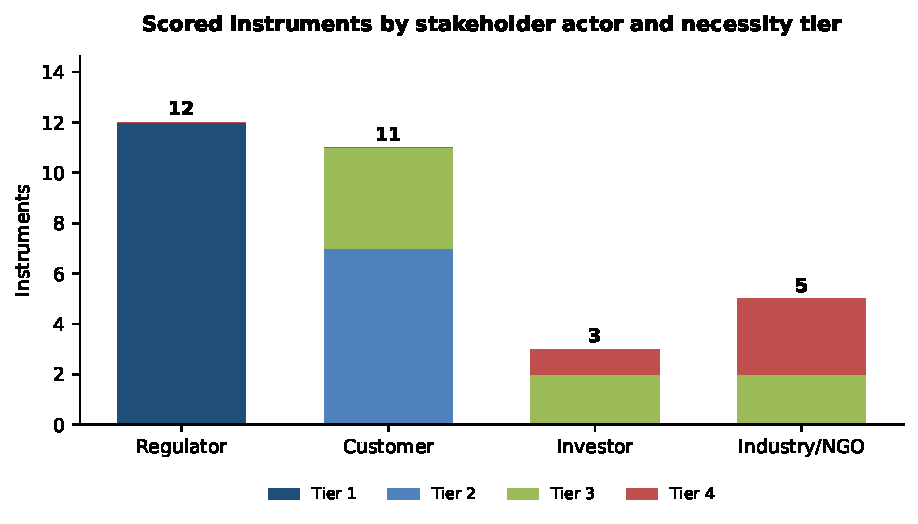
\includegraphics[width=0.78\linewidth]{r_actor_tier.pdf}
\caption{Composition of the scored demand environment: the 31 instrument columns
by stakeholder channel and necessity tier. Regulators and customers dominate;
investors are the thinnest channel.}
\label{fig:r-actor-tier}
\end{figure}

\FloatBarrier
\subsection{6.6 Narrow law, broad cascade}\label{cm-narrow-broad}

A second pattern concerns not \emph{who} demands but how \emph{broadly} each
instrument demands, and it reframes the SME's problem. Individual regulations are
narrow: each of the twelve regulatory instruments touches on average only two
topics, and none more than three - the Packaging and Packaging Waste Regulation
covers waste and packaging, the occupational-health directive covers health and
safety, the F-gas Regulation covers emissions. Breadth - and therefore the
overlap that creates the SME's burden - comes overwhelmingly from the market and
voluntary side: customer instruments demand on average nine topics each (the CSDDD
eighteen), and industry and NGO reporting frameworks almost eight (GRI alone
twenty-five).

The wall of overlapping demand is therefore not the product of the SME being
directly over-regulated. It is the product of a few \emph{broad} horizontal
instruments - CSRD, CSDDD, SFDR - that apply to the firm's large customers and
financiers and \emph{cascade} down the value chain as supplier questionnaires,
together with the voluntary certification and rating landscape. Direct regulation
on the processor is targeted and lean; the breadth is transmitted, not imposed.
This has a direct consequence for what an SME should do. The broad horizontal
instruments that generate the cascade - CSRD and its ESRS - are also, ultimately,
the most \emph{comprehensive} statement of what will be asked: a firm fully aligned
to the ESRS would, for the general-sustainability topics, already hold almost
everything a customer or financier could cascade down to it. Full ESRS alignment is
therefore the sensible end-state. But it is a large ask for a resource-constrained firm,
and in the interim the demand actually placed on SMEs is being deliberately capped - by the VSME and by the Omnibus value-chain provisions - to a proportionate
subset. The pragmatic path this chapter identifies sits between the two: rather than
attempt full alignment at once or simply wait for the caps to settle, a firm builds
first the \emph{most convergent} ESRS topics - those the demand mapping shows are
asked across the most channels - which are exactly the topics that secure its
licence to operate and to sell today, while laying ESRS-aligned foundations it can
extend, topic by topic, toward the fuller proactive posture. The same structure
carries a policy corollary, developed in the discussion: because the burden
originates in the downward cascade of large-firm regulation rather than in narrow
direct rules, it is the coordination and capping of that cascade - the aim of the
VSME and the Omnibus - that would most reduce it.
\FloatBarrier
\subsection{6.7 The build-first set by production
system}\label{cm-build-first}

Because several seafood instruments and topics are production-system-specific, the
diagnostic returns a different Stage-1 (build-first) set depending on whether the
firm is wild-capture, aquaculture, or both (Figure~\ref{fig:r-stage-system}). For
the standard modelled profile the Stage-1 set is nine topics for a mixed-sourcing
firm, eight for an aquaculture-only firm, and five for a wild-capture-only firm.

The \emph{overlap} is a universal core of four topics that should be build-first under
every production system: energy (E1-5), greenhouse-gas emissions (E1-6),
biodiversity and ecosystems (E4), and supply-chain traceability. These are the
no-regret priorities for any European seafood processor - demanded broadly,
across stakeholder channels, irrespective of business model.

Traceability is also the cheapest of the four to build, which is why it heads the
sequence rather than merely appearing in it. Most European processors already
hold BRCGS or IFS certification, and both require full traceability and chain of
custody as a condition of the certificate (BRCGS, 2022, clause~3.9; IFS
Management GmbH, 2023, requirement~4.18). The underlying records therefore
largely exist before any sustainability requirement is raised; what is usually
missing is not the data but its organisation for external reporting. Meeting the
MSC or ASC chain-of-custody requirement on top of an existing BRC or IFS system
is correspondingly less burdensome than its position in the demand matrix might
suggest. This is the build-once case in its clearest form: the topic with the
broadest demand across the ecosystem is also among the least costly to
supply.\footnote{This point was raised by a reviewer with sector experience and
is reflected here; see also the traceability systems reported by the cohort in
Table~\ref{tab:sector-material-evidence}.}

The \emph{differences} are structured rather than arbitrary. Four further
topics - water (E3-4), waste (E5-5), occupational health and safety (S1-14) and
value-chain workers (S2-1) - are Stage~1 for mixed and aquaculture firms but slip
to Stage~2 for a wild-capture firm. This is a volume effect, not a change in
importance. The matrix carries three aquaculture certifications (ASC, BAP,
GLOBALG.A.P.) against two wild ones (MSC, Friend of the Sea), so a wild-only firm
loses the certification demand that lifts these shared topics over the breadth
threshold. Their cross-stakeholder convergence is unchanged, and several retain a
regulatory floor (OSH, the Forced Labour Regulation, PPWR).

The counts follow from this. Four core topics plus these four give the eight of an
aquaculture-only firm; wild-stock sourcing joins them for a mixed firm, giving
nine. A wild-capture firm keeps the four core topics plus wild-stock sourcing, and
five is its total. Feed and animal health/antimicrobial use are scored for
aquaculture and mixed firms, but reach only Stage~2 and Stage~3 respectively,
which is why they do not add to the Stage-1 count. The personalisation therefore refines \emph{which} of a shared backbone
a firm should prioritise; it does not produce wholly different agendas for
different firms.

\begin{figure}[htbp]
\centering
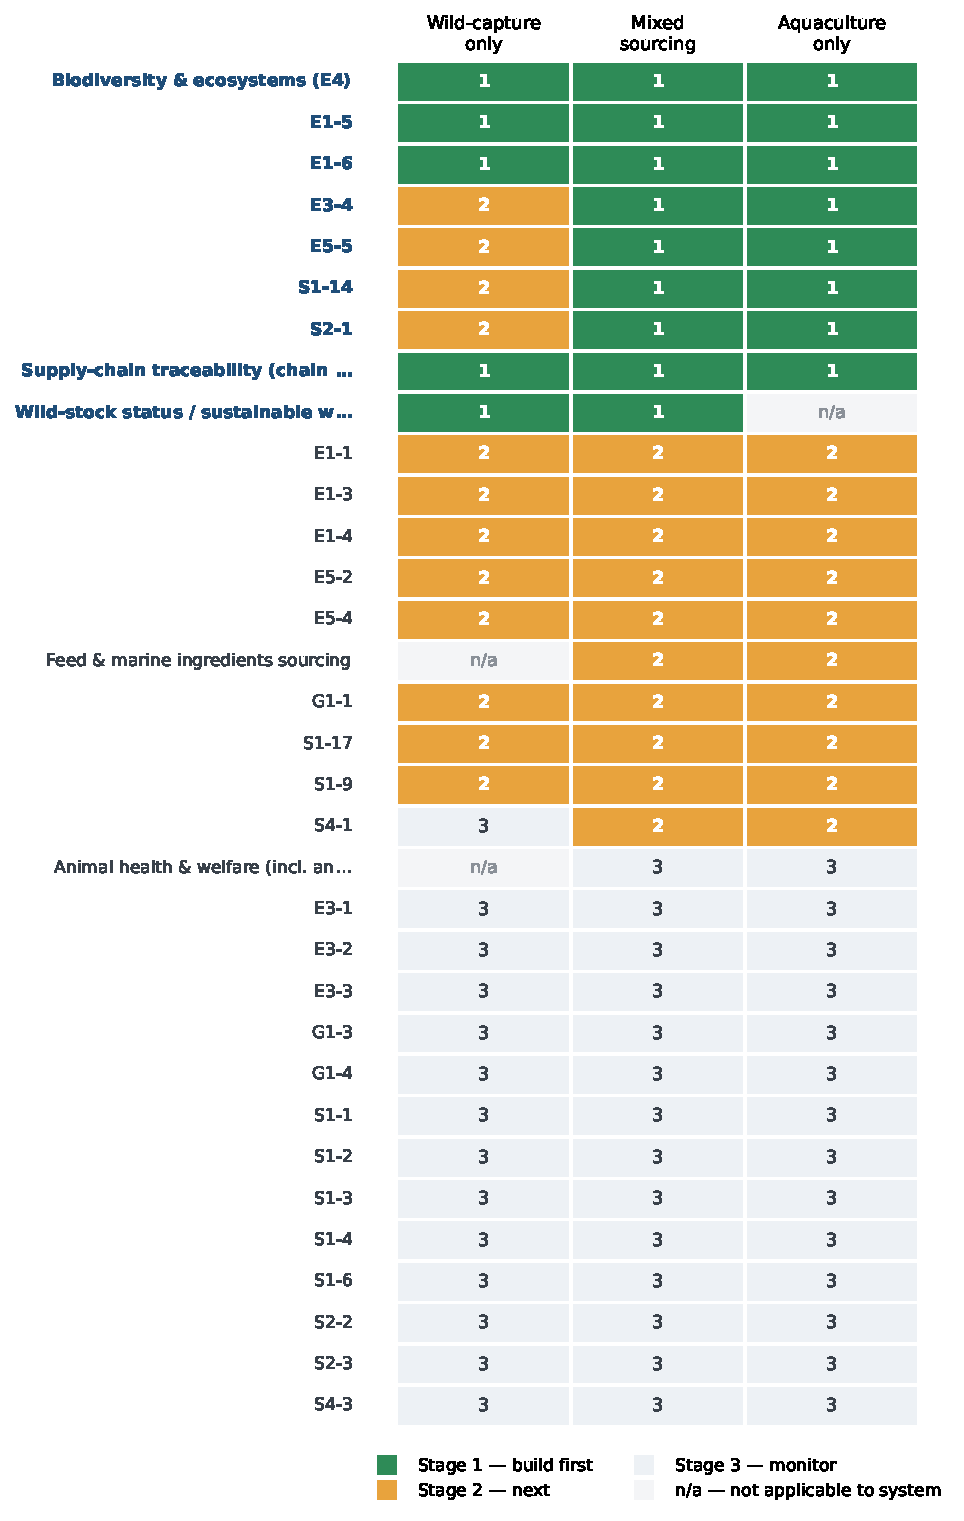
\includegraphics[width=0.56\linewidth]{r_stage_system.pdf}
\caption{First action points by production system. Each topic's stage
(1~=~build first, 2~=~next, 3~=~monitor) under a wild-only, mixed and
aquaculture-only profile; ``--'' marks a topic not applicable to that system. The
four topics that are Stage~1 across all systems form the universal core.}
\label{fig:r-stage-system}
\end{figure}

\FloatBarrier
\subsection{6.8 Step 4: from themes to datapoints, and the diagnostic
tool}\label{cm-datapoints-tool}

\textbf{The build-first data layer.} The staging returns priority \emph{themes};
a firm still needs to know which \emph{datapoints} to collect for each. A
datapoint layer translates every priority theme into the specific data the firm
must produce. The ESRS topical requirements decompose into their constituent
datapoints (the ESRS datapoint catalogue under Commission Delegated Regulation
(EU) 2023/2772): the 26 DR-level Stage rows resolve to 356 official datapoints
and the two topic-level rows (E4, S4) to a further 152. For each theme the
\emph{proportionate} subset - the realistic starting point for a smaller
firm - is identified through the VSME-to-ESRS crosswalk (\nameref{app:crosswalk}),
which maps every VSME Basic and Comprehensive module datapoint to the ESRS
disclosure requirement it is thematically closest to and flags whether it is
realistically self-reportable without external verification.
The crosswalk operates at disclosure-requirement level, not at official-datapoint
level: no ESRS datapoint is itself tagged as a starting point, but a VSME
datapoint mapped onto a theme's requirement shows that a lighter, self-assessable
version of that requirement exists. Applied to the Stage-1 set, five of the seven
ESRS-anchored topics have solid VSME coverage - energy, GHG emissions, water,
waste, and health and safety. Biodiversity is covered only partially, and
value-chain workers (S2-1) not at all. This confirms at datapoint resolution the
gap already identified in \nameref{app:esrs-mapping}. The four seafood-specific
themes have no ESRS requirement and are sourced from GRI~13, so they correctly
have no VSME entry either.

\textbf{The enabling layer.} Knowing which datapoints to collect is not the same
as knowing how to produce them. Each topic therefore also carries the enabling
instruments that generate its data - the GHG Protocol for emissions accounting,
GDST for traceability, ISO~14001 for environmental management. These are methods
and management systems rather than disclosure demands, which is why they are held
outside the demand sums (Section~6.3). Eight of the nine Stage-1 topics
carry at least one enabling instrument; biodiversity is the exception, with no
established method specific enough to name, which is consistent with its partial
VSME coverage and with its being the topic where demand most clearly outruns
practice (Section~7.1).

Each \emph{topic} (not datapoint) carries the count of stakeholder demands it
serves, taken from the matrix (Section~6.4). This makes the reuse
explicit: a single topic typically satisfies several frameworks at once. Because
both the ESRS and the VSME are under active Omnibus revision, the layer is a dated
snapshot documented with its sources.

\textbf{The diagnostic tool.} The staging logic is operationalised as a working
prototype for an individual SME. The tool takes two inputs the firm can supply
directly. The first is a short reporting-posture self-assessment of five to eight
items: whether it has a formal sustainability strategy, a dedicated function or
role, externally or internally initiated reporting, voluntary commitments such as
SBTi-aligned targets, and disclosure data that is reusable across requests. The
second is its production profile - wild, aquaculture or mixed, and size band. It
returns the firm's Stage-1 build-first topics filtered to that profile, and the
datapoint layer beneath them. This is the core of the diagnostic: it turns the
general staging into a personalised shortlist.

Two extensions are designed but not yet built into the prototype, and are described
here as the intended next increment. The first is a \emph{stakeholder-pressure
input}: the firm would identify which customers, certifications and investors are
actively asking, so the shortlist could be narrowed further to the topics where its
\emph{actual} demand and the convergent topics coincide. The second is a fully
automated \emph{staged roadmap} sequencing Stage~1~$\rightarrow$~2~$\rightarrow$~3
against the firm's posture and resourcing. Positioning on the reactive-to-proactive
spectrum is left to the self-assessment, on the basis that posture is a behavioural
rather than a measurable categorical state that the firm is best placed to judge.

\FloatBarrier
\subsection{6.9 Step 4 continued: worked case and
validation}\label{cm-worked-case}
% Scoping note: validating the diagnostic against a named real firm is
% deliberately left as a specified next step rather than attempted within
% this thesis -- a considered scope decision, not an oversight. Confirmed
% with Ruben (2026-07-24) to keep this framing given the send timeline.

\textbf{Worked case: scope and next step.} Validating the diagnostic against
a real firm's public disclosures is the natural empirical next step after
this thesis, and is deliberately scoped here as specified future work rather
than attempted under this thesis's time constraints. The design is specified
precisely enough to be immediately actionable: a representative European
mid-sized seafood-processing SME (50--250 employees, primarily a B2B
supplier to large EU retailers) would be profiled using only material the
firm has itself published - its sustainability report, certification
listings, and customer and product information - so the exercise depends
on no privileged access and is fully reproducible by a future researcher or
practitioner without a partner firm's cooperation. The diagnostic would be
run on that profile, and its output examined for correspondence to the
firm's observable position: whether it locates the firm's posture plausibly,
and whether the topics it flags as build-first match the demands the firm is
visibly subject to. By design the case is singular and \emph{formative rather
than confirmatory} - a usability demonstration of the diagnostic, not a
test of the underlying empirical claims about the cohort or the
cross-framework demand pattern - and no generalisation beyond it would be
claimed. Practitioner validation of the diagnosis with the firm itself is a
further, separate step, identified here and left to future work regardless
of whether the worked case is carried out first.

Figure~\ref{fig:tool-screenshot} shows the diagnostic's actual output screen,
illustrating the format this validation step would use. The profile shown sits
within the scoped parameters - mixed wild-plus-aquaculture sourcing, sub-250
employees - rather than belonging to a named firm. Given a production profile,
the tool returns a ranked Stage-1 build-first set and states how much of the
demand environment building it answers. A firm therefore sees not only
\emph{what} to build first but \emph{why that subset}.

\begin{figure}[htbp]
\centering
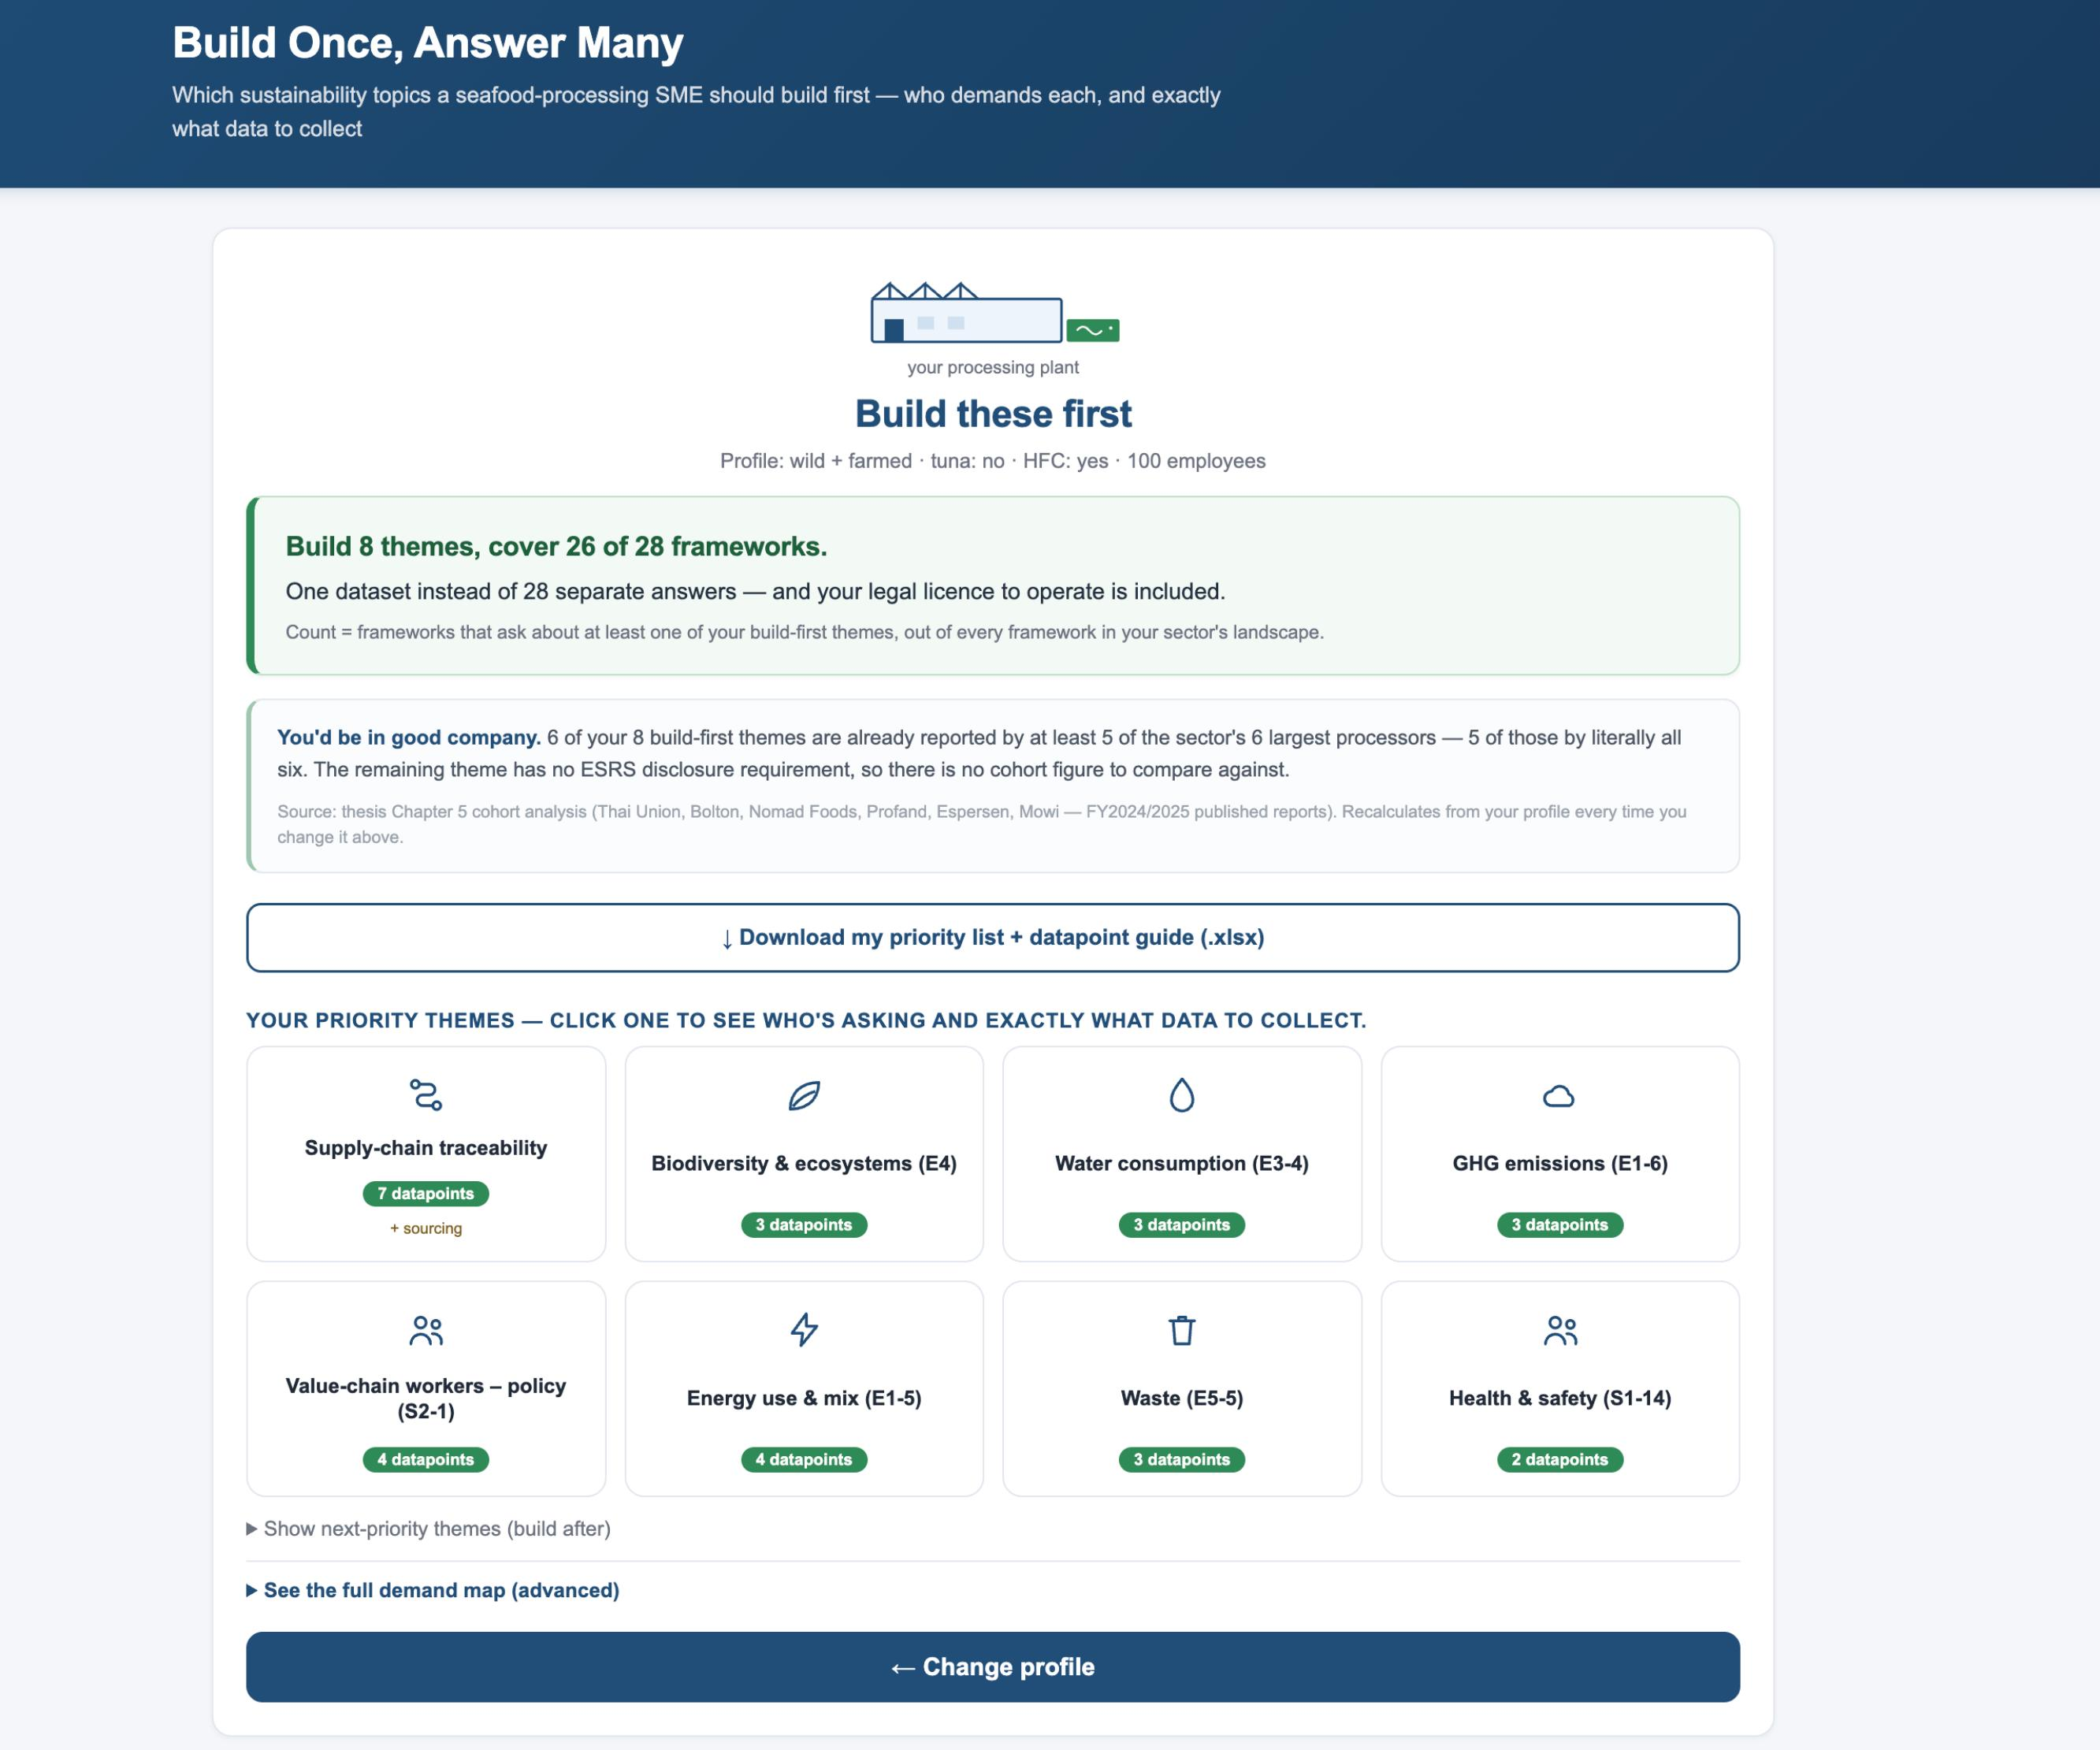
\includegraphics[width=\linewidth]{phase3/tool.jpg}
\caption{The diagnostic tool's output screen: for a given production
profile, it returns the ranked Stage-1 (build-first) themes, the
datapoints each requires, and the share of the sector's demand environment
they jointly answer. This is the operational form the
staging logic of Section~6.4 takes for an individual firm. The mixed profile
shown returns nine Stage-1 topics but eight tiles, because the tool presents
wild-stock sourcing within supply-chain traceability - the two are evidenced
by one set of chain-of-custody data.}
\label{fig:tool-screenshot}
\end{figure}

\textbf{Validation of the mapping and the mechanism.} Both the demand mapping and
the capability-sharing claim beneath it are substantiated from documents, so that
credibility rests on independently inspectable evidence rather than on any single
informant.

The \emph{descriptive} claim is that the ecosystem can be organised exhaustively
and unambiguously by the necessity, domain and source axes. Its test is the
completeness of the classification itself, every instrument placed and every
placement reasoned. The classification has also been submitted to the
sustainability leads at the cohort firms for member checking (Lincoln \& Guba,
1985); that corroboration is outstanding at the time of writing.

The \emph{explanatory} claim is that capabilities are shared across requirements,
so that investment compelled by a lower-tier requirement subsidises higher-tier
disclosure. This is substantiated through an \emph{input-overlap analysis}: for
each shared capability, the inputs the drawing instruments require are read
directly from their published specifications. MSC chain-of-custody, the GDST
standard and ESRS value-chain disclosure all draw on the same body of lot-level
traceability data - shared inputs that are document-verifiable rather than
self-reported.

The evidence is therefore \emph{consistent with} the capability-sharing mechanism;
it does not prove a causal relationship. Establishing that would take retrospective
practitioner testimony on whether capability built for a mandatory requirement
reduced the effort of later disclosures. That is the natural next stage, and is
left to future work.

\medskip
The implications for seafood SMEs and for EU disclosure policy are drawn out
in the discussion that follows.
